\documentclass[a4]{article}
\pagestyle{myheadings}

%%%%%%%%%%%%%%%%%%%
% Packages/Macros %
%%%%%%%%%%%%%%%%%%%
\usepackage{mathrsfs}


\usepackage{fancyhdr}
\pagestyle{fancy}
\lhead{}
\chead{}
\rhead{}
\lfoot{}
\cfoot{} 
\rfoot{\normalsize\thepage}
\renewcommand{\headrulewidth}{0pt}
\renewcommand{\footrulewidth}{0pt}
\newcommand{\RomanNumeralCaps}[1]
    {\MakeUppercase{\romannumeral #1}}

\usepackage{amssymb,latexsym}  % Standard packages
\usepackage[utf8]{inputenc}
\usepackage[russian]{babel}
\usepackage{MnSymbol}
\usepackage{mathrsfs}
\usepackage{amsmath,amsthm}
\usepackage{indentfirst}
\usepackage{graphicx}%,vmargin}
\usepackage{graphicx}
\graphicspath{{pictures/}} 
\usepackage{verbatim}
\usepackage{color}
\usepackage[nottoc,numbib]{tocbibind}
\usepackage{float}

\usepackage{listings}
\definecolor{codegreen}{rgb}{0,0.6,0}
\definecolor{codegray}{rgb}{0.5,0.5,0.5}
\definecolor{codepurple}{rgb}{0.58,0,0.82}
\definecolor{backcolour}{rgb}{0.95,0.95,0.92}
 
\lstdefinestyle{mystyle}{
    backgroundcolor=\color{backcolour},   
    commentstyle=\color{codegreen},
    keywordstyle=\color{magenta},
    numberstyle=\tiny\color{codegray},
    stringstyle=\color{codepurple},
    basicstyle=\footnotesize,
    breakatwhitespace=false,         
    breaklines=true,                 
    captionpos=b,                    
    keepspaces=true,                 
    numbers=left,                    
    numbersep=5pt,                  
    showspaces=false,                
    showstringspaces=false,
    showtabs=false,                  
    tabsize=2
}
 
\lstset{style=mystyle}

\usepackage{url}
\urldef\myurl\url{foo%.com}





\DeclareGraphicsExtensions{.pdf,.png,.jpg}% -- настройка картинок

\usepackage{epigraph} %%% to make inspirational quotes.
\usepackage[all]{xy} %for XyPic'a
\usepackage{color} 
\usepackage{amscd} %для коммутативных диграмм
%\usepackage[colorlinks,urlcolor=red]{hyperref}

%\renewcommand{\baselinestretch}{1.5}
%\sloppy
%\usepackage{listings}
%\lstset{numbers=left}
%\setmarginsrb{2cm}{1.5cm}{1cm}{1.5cm}{0pt}{0mm}{0pt}{13mm}


\newtheorem{Lemma}{Лемма}[section]
\newtheorem{Proposition}{Предложение}[section]
\newtheorem{Theorem}{Теорема}[section]
\newtheorem{Corollary}{Следствие}[section]
\newtheorem{Remark}{Замечание}[section]
\newtheorem{Definition}{Определение}[section]
\newtheorem{Designations}{Обозначение}[section]




%%%%%%%%%%%%%%%%%%%%%%% 
%Подготовка оглавления% 
%%%%%%%%%%%%%%%%%%%%%%% 
\usepackage[titles]{tocloft}
\renewcommand{\cftdotsep}{2} %частота точек
\renewcommand\cftsecleader{\cftdotfill{\cftdotsep}}
\renewcommand{\cfttoctitlefont}{\hspace{0.38\textwidth} \LARGE\bfseries} 
\renewcommand{\cftsecaftersnum}{.}
\renewcommand{\cftsubsecaftersnum}{.}
\renewcommand{\cftbeforetoctitleskip}{-1em} 
\renewcommand{\cftaftertoctitle}{\mbox{}\hfill \\ \mbox{}\hfill{\footnotesize Стр.}\vspace{-0.5em}} 
%\renewcommand{\cftchapfont}{\normalsize\bfseries \MakeUppercase{\chaptername} } 
%\renewcommand{\cftsecfont}{\hspace{1pt}} 
\renewcommand{\cftsubsecfont}{\hspace{1pt}} 
%\renewcommand{\cftbeforechapskip}{1em} 
\renewcommand{\cftparskip}{3mm} %определяет величину отступа в оглавлении
\setcounter{tocdepth}{5} 
\renewcommand{\listoffigures}{\begingroup %добавляем номер в список иллюстраций
\tocsection
\tocfile{\listfigurename}{lof}
\endgroup}
\renewcommand{\listoftables}{\begingroup %добавляем номер в список иллюстраций
\tocsection
\tocfile{\listtablename}{lot}
\endgroup}


   
   
%\renewcommand{\thelikesection}{(\roman{likesection})}
%%%%%%%%%%%
% Margins %
%%%%%%%%%%%
\addtolength{\textwidth}{0.7in}
\textheight=630pt
\addtolength{\evensidemargin}{-0.4in}
\addtolength{\oddsidemargin}{-0.4in}
\addtolength{\topmargin}{-0.4in}

%%%%%%%%%%%%%%%%%%%%%%%%%%%%%%%%%%%
%%%%%%Переопределение chapter%%%%%% 
%%%%%%%%%%%%%%%%%%%%%%%%%%%%%%%%%%%
\newcommand{\empline}{\mbox{}\newline} 
\newcommand{\likechapterheading}[1]{ 
\begin{center} 
\textbf{\MakeUppercase{#1}} 
\end{center} 
\empline} 

%%%%%%%Запиливание переопределённого chapter в оглавление%%%%%% 
\makeatletter 
\renewcommand{\@dotsep}{2} 
\newcommand{\l@likechapter}[2]{{\bfseries\@dottedtocline{0}{0pt}{0pt}{#1}{#2}}} 
\makeatother 
\newcommand{\likechapter}[1]{ 
\likechapterheading{#1} 
\addcontentsline{toc}{likechapter}{\MakeUppercase{#1}}} 




\usepackage{xcolor}
\usepackage{hyperref}
\definecolor{linkcolor}{HTML}{000000} % цвет ссылок
\definecolor{urlcolor}{HTML}{AA1622} % цвет гиперссылок
 
\hypersetup{pdfstartview=FitH,  linkcolor=linkcolor,urlcolor=urlcolor, colorlinks=true}

%%%%%%%%%%%%
% Document %
%%%%%%%%%%%%

%%%%%%%%%%%%%%%%%%%%%%%%%%%%%
%%%%%%главы -- section*%%%%%%
%%%%section -- subsection%%%%
%subsection -- subsubsection%
%%%%%%%%%%%%%%%%%%%%%%%%%%%%%
\def \newstr {\medskip \par \noindent} 



\begin{document}
\def\contentsname{\LARGE{Содержание}}
\thispagestyle{empty}
\begin{center} 
\vspace{2cm} 
{\Large \sc Санкт-Петербургский Политехнический}\\
\vspace{2mm}
{\Large \sc Университет} им. {\Large\sc Петра Великого}\\
\vspace{1cm}
{\large \sc Институт прикладной математики и механики\\ 
\vspace{0.5mm}
\textsc{}}\\ 
\vspace{0.5mm}
{\large\sc Кафедра прикладной математики}\\
\vspace{15mm}
%\rule[0.5ex]{\linewidth}{2pt}\vspace*{-\baselineskip}\vspace*{3.2pt} 
%\rule[0.5ex]{\linewidth}{1pt}\\[\baselineskip] 
{\huge \sc Лабораторная работа №$2$\\
\vspace{0.1cm}
Характеристики положения\\
\vspace{0.5cm}
выборки
\vspace{6mm}
 }
\vspace*{2mm}
%\rule[0.7ex]{\linewidth}{1pt}\vspace*{-\baselineskip}\vspace{3.2pt} 
%\rule[0.5ex]{\linewidth}{2pt}\\ 
\vspace{1cm}

{\sc $3$ курс$,$ группа $3630102/70301$}

\vspace{2cm} 
Студент \hfill Лебедев К.С.\\
\vspace{1cm}
Преподаватель \hfill Баженов А. Н.\\
\vspace{20mm} 

\end{center} 
%\author{Я}
\begin{center}
\vfill {\large\textsc{Санкт-Петербург}}\\ 
2020 г.
\end{center}

%%%%%%%%%%%%%%%%%%%%%%%%%%%%%%%%%%%%%%%%%%%%%%%%%%%%%%%%%%%%%%%%%%%%%%%%%%%%%%%%%%%%%%%%%%%%%%
%\ \\[4cm]

%\rm
%%%%%%%%%%%%%%%%%%%%%%%%%%%%%%%%%%%%%%%%%%%%%%%%%%%%%%%%%%%%%%%%%%%%%%%%%%%%%%%%%%%%%%%%%%%%%%
\newpage
\pagestyle{plain}

%\begin{center}
%\begin{abstract} 

%\end{abstract}

%\end{center}

\newpage
\tableofcontents{}
\newpage

\section{Постановка задачи}

Cгенерировать выборки размеров $20,$ $60,$ $100$ элементов для $5$ти распределений. Для каждой выборки вычислить $\overline{x},\; med\; x,\; Z_R,\; Z_Q,\; Z_{tr},$ при $r = \frac{n}{4}.$

Распределения:
\begin{itemize}
\item Стандартное нормальное распределение
\item Стандартное распределение Коши
\item Распределение Лапласа 
\item Равномерное распределение 
\item Распределение Пуассона 
\end{itemize}



\section{Теория}

\begin{enumerate}
\item Выборочное среднее \cite{average}:
\begin{equation}\label{eqn:average}
\overline{x} = \frac{1}{n}\sum_{i=1}^n x_i \hfill  
\end{equation}
\item Выборочная медиана \cite{med}:
\begin{equation}
med\; x = \begin{cases}
x_{k+1}, & n = 2k+1\\
\frac{1}{2}\left(x_k+x_{k+1}\right), & n = 2k
\end{cases} \hfill  \label{eqn:med}
\end{equation}
\item Полусумма экстремальных значений \cite{mean_extr}:
\begin{equation}
Z_R = \frac{1}{2}\left(x_1+x_n\right) \hfill  \label{eqn:mean_extr}
\end{equation}
\item Полусумма квартилей \cite{quartiles}:
\begin{equation}
Z_Q = \frac{1}{2}\left(Z_{\frac{1}{4}}+Z_{\frac{3}{4}}\right) \hfill  \label{eqn:quartiles}
\end{equation}
\item Усечённое среднее \cite{cut_mean}:
\begin{equation}
Z_{tr} = \frac{1}{n - 2r}\sum_{i=r+1}^{n-r} x_i \hfill  \label{eqn:cut_mean}
\end{equation}
\end{enumerate}

\section{Реализация}
Для генерации выборки был использован $Python\;3.6$: модуль $random$ библиотеки $numpy$ \cite{numpy} для генерации случайных чисел с различными распределениями. Также с помощью библиотеки $numpy$ были вычислены характеристики положения.

После вычисления характеристик положения $1000$ раз находится среднее значение и дисперсия: 
\begin{equation}
E(z) = \frac{1}{n}\sum_{i=1}^n z_i
\end{equation} 
\begin{equation}
D(z) = E\left(z^2\right) - E^2(z)
\end{equation}



\newpage
\section{Результаты}

\begin{center}

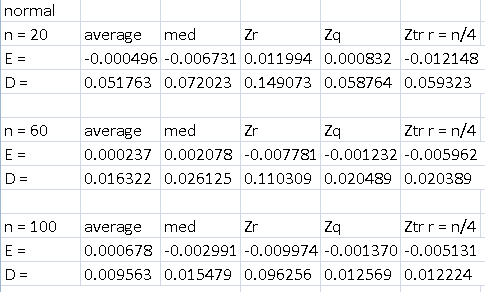
\includegraphics[width=\textwidth]{normal.png} \textbf{Нормальное распределение}
\vspace{50pt}

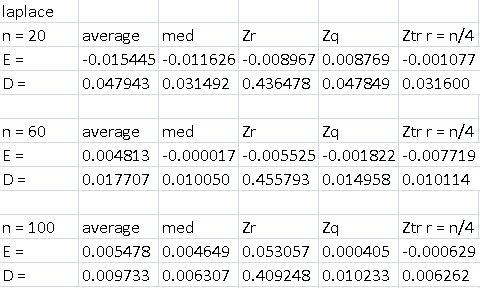
\includegraphics[width=\textwidth]{laplace.png} \textbf{Распределение Лапласа}\\
\vspace{50pt}

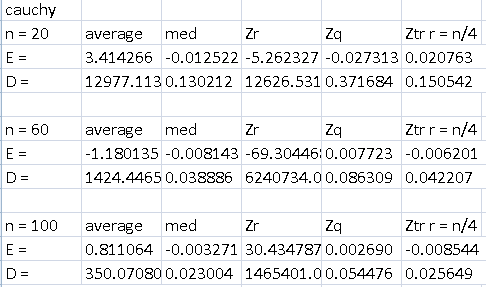
\includegraphics[width=\textwidth]{cauchy.png} \textbf{Распределение Коши }\\
\vspace{50pt}

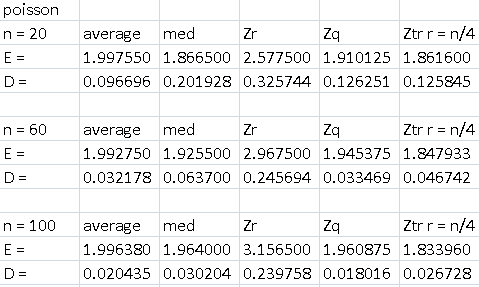
\includegraphics[width=\textwidth]{poisson.png} \textbf{Распределение Пуассона }\\
\vspace{50pt}

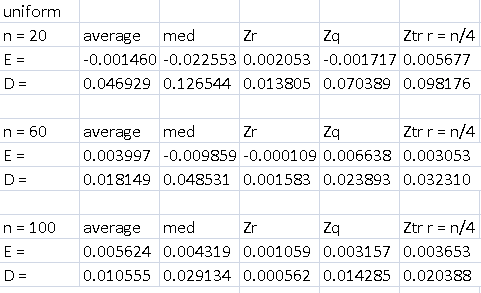
\includegraphics[width=\textwidth]{uniform.png} \textbf{Равномерное распределение }\\

\end{center}

\section{Выводы}

\par В процессе работы вычислены значения характеристик положения для определённых распределений на выборках разной мощности и получено следующее ранжирование характеристик положения:

\begin{enumerate}
    \item Стандартное нормальное распределение $$\overline{x} < Z_{tr} < Z_Q < med\;x < Z_R$$
    
    \item Стандартное распределение Коши $$med\;x < Z_Q < Z_{tr} < \overline{x} < Z_R$$
    
    \item Распределение Лапласа (коэффициент масштаба $\sqrt{2}$ коэффициент сдвига равен нулю) $$med\;x < Z_{tr} < \overline{x} < Z_Q < Z_R$$
    
    \item Равномерное распределение на отрезке $\left[-\sqrt{3},\sqrt{3}\right]$ $$Z_R < \overline{x} < Z_{tr} < Z_Q < med\;x$$
    
    \item Распределение Пуассона (значение мат ожидания равно $3$) $$\overline{x} < Z_{tr} < Z_Q < med\;x < Z_R$$
    
\end{enumerate}



\begin{thebibliography}{}
    \bibitem{numpy}  Модуль numpy  -  https://physics.susu.ru/vorontsov/language/numpy.html
    
    \bibitem{distr_formulas}  
    Формулы распределений  -  https://vk.com/doc184549949\_491827451
    
    \bibitem{average}  
    Выборочное среднее  -  https://en.wikipedia.org/wiki/Sample\_mean\_and\_covariance
    
    \bibitem{med}  
    Выборочная медиана  -  http://femto.com.ua/articles/part\_1/2194.html
    
    \bibitem{mean_extr}  
    Полусумма экстремальных значений  -  https://studopedia.info/8-56888.html
    
    \bibitem{quartiles}  
    Квартили  -  https://studfiles.net/preview/2438125/page:13/
    
    \bibitem{cut_mean}  Усечённое среднее  -  https://ole-olesko.livejournal.com/15773.html
\end{thebibliography}


\lstinputlisting[language=Python]{lab2.py}

\end{document}
